\documentclass[12pt,a4paper]{article}
\usepackage[utf8]{inputenc}
\usepackage[spanish]{babel}
\usepackage{amsmath}
\usepackage{amsfonts}
\usepackage{amssymb}
\usepackage{graphicx}
\usepackage{float}
\usepackage{caption}
\usepackage[left=2cm,right=2cm,top=2cm,bottom=2cm]{geometry}
\usepackage{multicol}
\author{Tatiana Dávila Egas}
\title{Modelo Atómico de Bohr}
\date{}
\begin{document}
\maketitle
\section{Introducción}
-<B<YJNH-O<SB-V<G-LHSV<-NL<HC-KVSJBLEBÑLJWEBC<BKL<
\begin{figure}[!ht]
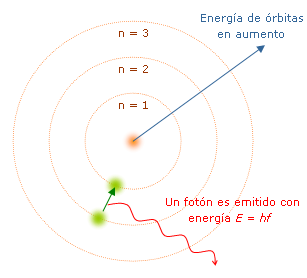
\includegraphics[scale=0.6]{Modelo_de_Bohr.png}
\centering 
\caption{Diagrama del modelo\\ atómico de Bohr}
\end{figure}


\section{Postulados de Bohr}
\begin{enumerate}
\item Primer postulado
Los electrones describen órbitas circulares en torno al núcleo del átomo sin irradiar energía.

La causa de que el electrón no irradie energía en su órbita es, de momento, un postulado, ya que según la electrodinámica clásica una carga con un movimiento acelerado debe emitir energía en forma de radiación.

Para mantener la órbita circular, la fuerza que siente el electrón —la fuerza coulombiana por la presencia del núcleo— debe ser igual a la fuerza centrípeta. Esto nos da la siguiente expresión:

\begin{equation}
r=k\dfrac{Ze^{2}}{m_{e}v^{2}}
\end{equation}
Y ahora, con esta ecuación, y sabiendo que la energía total es la suma de las energías cinética y potencial:
\begin{equation}
E=T+V=\dfrac{1}{2}m_{e}v^{2}-k\dfrac{Ze^{2}}{r}=-\dfrac{1}{2}\dfrac{kZe^{2}}{r}
\end{equation}
Donde queda expresada la energía de una órbita circular para el electrón en función del radio de dicha órbita.


\item Segundo postulado

\begin{multicols}{2}
No toda órbita para electrón está permitida, tan solo se puede encontrar en órbitas cuyo radio cumpla con el momento angular, $L$, del electrón sea un múltiplo entero de $\hbar=\dfrac{h}{2\pi}$ Esta condición matemáticamente se escribe: $$L=m_{e}vr=n\hbar$$ con $n= 1,2,3...$.\\ A partir de ésta condición y de la expresión para el radio obtenida antes, podemos eliminar $v$ y queda la condición de cuantización para los radios permitidos:
$$r_{n}=\dfrac{n^{2}\hbar^{2}}{km_{e}Ze^{2}}$$ con $n= 1,2,3\ldots$  \ .
\begin{center}
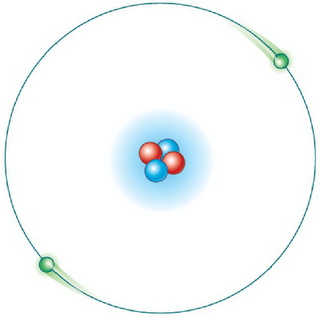
\includegraphics[scale=.4]{MODELO_ATOMICO_DE_BOHR2pos.png}
\end{center}
\end{multicols}


\item Tercer postulado 
\begin{multicols}{2}

\begin{center}
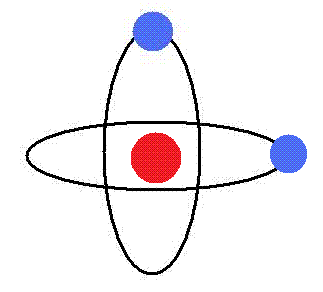
\includegraphics[scale=0.5]{Bohr-model3pos.png} 
\end{center}
El electrón solo emite o absorbe energía en los saltos de una órbita permitida a otra. En dicho cambio emite o absorbe un fotón cuya energía es la diferencia de energía entre ambos niveles. Este fotón, según la ley de Planck tiene una energía: $$E_{\gamma}=hv=E_{nf}-E_{ni}$$ 
    donde $n_i$ identifica la órbita inicial y $n_f$ la final, y $\nu$ es la frecuencia.\\
Entonces las frecuencias de los fotones emitidos o absorbidos en la transición serán:
$$v=\dfrac{k^{2}m_{e}Z^{2}e^{4}}{2h\hbar^{2}}\left( \dfrac{1}{n^{2}_i}-\dfrac{1}{n^{2}_{i}}\right)$$
Se puede demostrar que este conjunto de hipótesis corresponde a la hipótesis de que los electrones estables orbitando un átomo están descritos por funciones de onda estacionarias. Un modelo atómico es una representación que describe las partes que tiene un átomo y como están dispuestas para formar un todo. Basándose en la constante de Planck $E=hv$, consiguió cuantizar las órbitas observando las líneas del espectro.
\end{multicols}
\end{enumerate}

\end{document}